\documentclass[a4paper]{article}
%\usepackage{fourier-otf}
\usepackage[utf8]{inputenc}
\usepackage{graphicx}
\usepackage{algorithm}
\usepackage{algpseudocode}
\usepackage{float}
\usepackage{lipsum}
\usepackage{scrextend}
\usepackage{biblatex}
\addbibresource{bibliography.bib}
\usepackage{listings}
\usepackage{amsmath}
\usepackage{amsfonts}
%\usepackage[square,sort,comma,numbers]{natbib}
\newtheorem{theorem}{Theorem}[section]
\usepackage{color}
\usepackage{makeidx}
\usepackage{titlepic}
\definecolor{mygreen}{rgb}{0,0.6,0}
\definecolor{mygray}{rgb}{0.5,0.5,0.5}
\definecolor{mymauve}{rgb}{0.58,0,0.82}
\lstset{ %
	backgroundcolor=\color{white},   % choose the background color
	basicstyle=\footnotesize,        % size of fonts used for the code
	breaklines=true,                 % automatic line breaking only at whitespace
	captionpos=b,                    % sets the caption-position to bottom
	commentstyle=\color{mygreen},    % comment style
	escapeinside={\%*}{*)},          % if you want to add LaTeX within your code
	keywordstyle=\color{blue},       % keyword style
	stringstyle=\color{mymauve},     % string literal style
}
\usepackage{hyperref}
\hypersetup{
  colorlinks   = true,    % Colours links instead of ugly boxes
  urlcolor     = black,    % Colour for external hyperlinks
  linkcolor    = black,    % Colour of internal links
  citecolor    = black      % Colour of citations
}
%\title{First chapter}

%\author{F.Bernardi}

%\protect\\ 

\newcommand{\myName}{Fabrizio Bernardi}
\newcommand{\myTitle}{Modeling and data analysis of the calcium activity in somatostatin interneurons from in vivo imaging on mice }
\newcommand{\myDegree}{Programme: \protect\\ \textit{Mathematical Engineering}}
\newcommand{\myCycle}{XXXI cycle}
\newcommand{\myDepartment}{Department of Mathematics}
\newcommand{\myUni}{Politecnico di Milano}
\newcommand{\myYear}{2022}
\newcommand{\myTime}{01 Jan \myYear}

\pdfbookmark{Cover}{cover}

\begin{document}
	
	
	
\section{Interbrain data analysis: emotion discrimination task}

In this second chapter, the main results on the data analysis on the emotion discrimination task are presented. After describing the phases of the task and trying to understand whcih an be an appropriate way  to represent the data, through normalizations, first results on the neural activity of mice in relation to their behaviour are presented. Then, the focus goes on the main part of the analysis: the interbrain synchrony between such activities. The different concepts of synchrony introduced in Chapter 2 habe been investigated, such as the study of causality between signal via Granger prediction. 


\subsection{Emotion discrimination task}

\begin{figure}[H]
	\begin{center}
		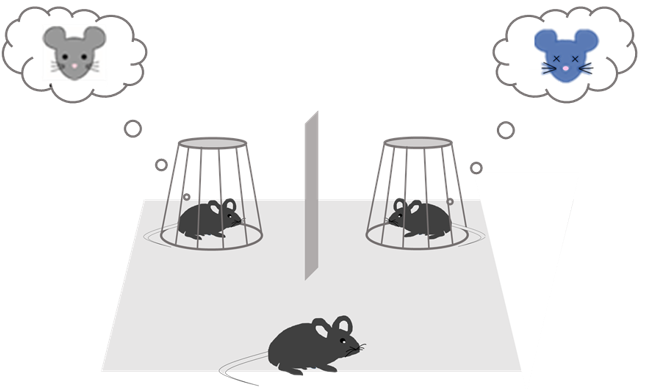
\includegraphics[scale=.90]{emotion_discrimination.png} 
	\end{center} 
	\caption{\textit{Scheme of the emotion discrimination task}}
	
\end{figure}

The \textit{emotion discrimination task} consists of an observer mouse facing two demonstrators in an open arena. One demonstrator is in a \textit{neutral} state, the other in a \textit{stressed} state, i.e. it has been subjected to a \textit{stress protocol} (forced restrainment) before the test. The task consists of three main parts:

\begin{enumerate}
	
	\item \textbf{Homecage restrainment}: the three mice are kept separate in a cage in normal conditions. \\
	$\longrightarrow$ \textit{Duration}: 5 minutes
	
	\item \textbf{Habituation}: the observer mouse is free to move in an empty open arena; in the meantime the neutral demonstrator is kept in the cage, while the stressed demonstrator is being subjected to the stressing procedure \\
	$\longrightarrow$  \textit{Duration}: 15 minutes
	
	\item \textbf{Test}: the demonstrators join the observer in the arena. Only the observer is free to move, since the two demonstrators are kept behind a cage allowing sight, sniffing but no passage \\
	$\longrightarrow$  \textit{Duration}: 15 minutes
\end{enumerate}

During all the three phases, the neural activities of the three mice are recorded via microendoscopic calcium imaging as described in Section 1.3, in which the target are \textit{somatostating-expressing} interneurons in the anterior cingulate cortex (Section 1.1). Moreover, the position of the observer mouse along time is recorded during habituation and test phases, such as TTL signals (binary recording of events) of the reciprocal sniffing between one observer and a demonstrators have been measured during the test. Finally, spatial data of the neurons in the \textit{region of interest (ROI)} captured by the miniscope, are present as well, such as their position and size.\\
These type of data can lead to several analyses:
\begin{itemize}
	
	\item Inspecting if there are correlations between the neural activity levels of one mouse and what is happening during the task, such as the stressing procedure or the proximity of two mice
	
	\item Testing the presence of \textit{activity synchronization}, as described in Section 2.1-2.4, between the neural signals of two mice, in relation to what is happening in the test (proximity of two subjects, sniffing...)
	
	\item Investigating whether the activity in one mice is \textit{predicting} the activity in another, for example via a Granger causality analysis introduced in Section 2.5
	
	\item Wondering wether the neuronal firing in single mice seems to follow \textit{patterns}, or if it is possible to predict mathematically such chain of events (problem dealt in Chapter 7)
\end{itemize}
	
		
The analyses have been conducted on 3 different datasets, meaning that 3 triplets of mice tested with the same procedure. Moreover two more experiments have been performed in the so called \textbf{self-experience} setting, in which, before the test, also the observer is subjected to a stress protocol.\\
It is worth to stress the fact that the phases of homecage and habituation play the role of a \textit{control} in the data analysis: given a quantity measured from the data of calcium concentrations, we can assume that a result is significant, and thus related to the interactions between mice, if it is present in the test phase but not in the control phases of homecage and habituation, in which the mice cannot interact and are located in different places.

\subsection{Normalizing the dataset}
	
	
	\begin{figure}[H]
			
		\begin{center}
			\hspace*{-2.1cm}
			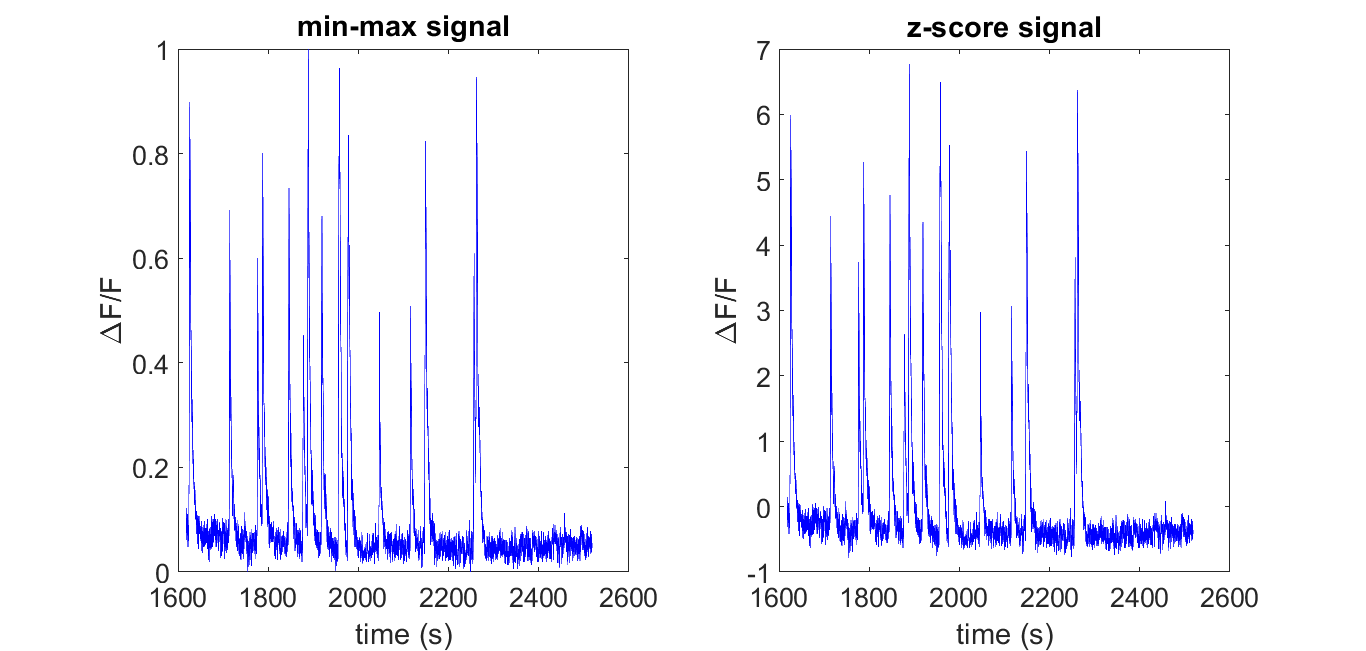
\includegraphics[scale=.45]{normalizations.png} 
		\end{center} 
		\caption{\textit{Left: min-max normalization, with signal in $[0,1]$. Right: z-score normalization, with no constrain on the scale. }}
		
	\end{figure}
The main objects of the analysis are the calcium tracks recorded in every single neurons, expressed in terms of relative fluorescence $\frac{\Delta F}{F}$. Such signals will be subjected to operations (such as mean) and comparisons, both between neurons of a single mouse, and between activities of different mice. It necesessarely follows that it is fundamental to determine a priori a \textit{normalization} of the data which can allow such processes. The literature proposes several ways to threat data, for example: (see Figure):

\begin{enumerate}
	
	\item \textbf{Raw approach}. The raw data, coming from the Inscopix pre-processing described in Section 1.4, are usually not ready to be analyzed yet. Although normalizations on the videos, filtering, nose detection process have been already performed, the single information of a fluorescence value $\frac{\Delta F}{F}$ needs to be threated carefully. Every single neuron is characterized by a baseline activity, alternated with rapid and huge calcium spikes. Such baseline value, even if biiologically represents in any case a non active neuron, can have difference values across neurons. Moreover, the value reached by every spike can be quite different across different neurons, but this not necessarely reflects the same difference in what is really happening in the neuron: a spike can be less marked for the simple fact that less GCaMP protein was present at that moment, and consequently the spiking of that neuron happened at a smaller scale, preserving however its shape. 
	
	\item \textbf{min-max normalization}. With the min-max normalization, every value $x_t$ of the signal $ x = \left\{ x_t\right\}_{t=1}^N$ at time $t$ is normalized through
	
	\begin{equation}
		x_t^{mm} = \frac{x_t -  \min(x)}{\max(x) - \min(x)}
	\end{equation}
	
	With the min-max normalization, all the signals are bounded in the iterval $[0,1]$, in which the limit values are assumed by the highest and lowest values, respectively. Therefore, using this normalization, all the signals are threated in the same way, since they are all uniformed in the same interval, whatever it was their original value.
	
	\item \textbf{z-score normalization}. For a value  $x_t$ of the signal $ x = \left\{ x_t\right\}_{t=1}^N$, the z-score normalization reads
	
	\begin{equation}
	x_t^{z} = \frac{x_t -  \mu}{\sigma}
	\end{equation}
	
	where $\mu$ and $\sigma$ are the mean and standard deviation of the signal, respecitively. The goal of this normalization is to bring every signal at mean $0$ and standard deviation $1$, making them more comparable without directly putting constrains on their values, as it was in the case of the min-max normalization


\end{enumerate}
	
	
	All the different normalization does not modify the shape, but they modify the \textit{scale} of the values. As for this work, the choice went on a normalization \textbf{z-score on baseline}, in which signals are aligned and then divided by their dìstandard deviations such as in the z-score case, but the alignment is not performed on their mean. The reason for this is that two signals of this type may have the same mean, but different baseline activities. Therefore, the alignment is done on such baselines, which are set to $0$ for every neuron.
	
	
	
	\subsection{Behavioural analyses of the task}
	
	
	\begin{figure}[H]
		
		%\begin{center}
		\centering
			
			\hspace*{-1.4 cm}
			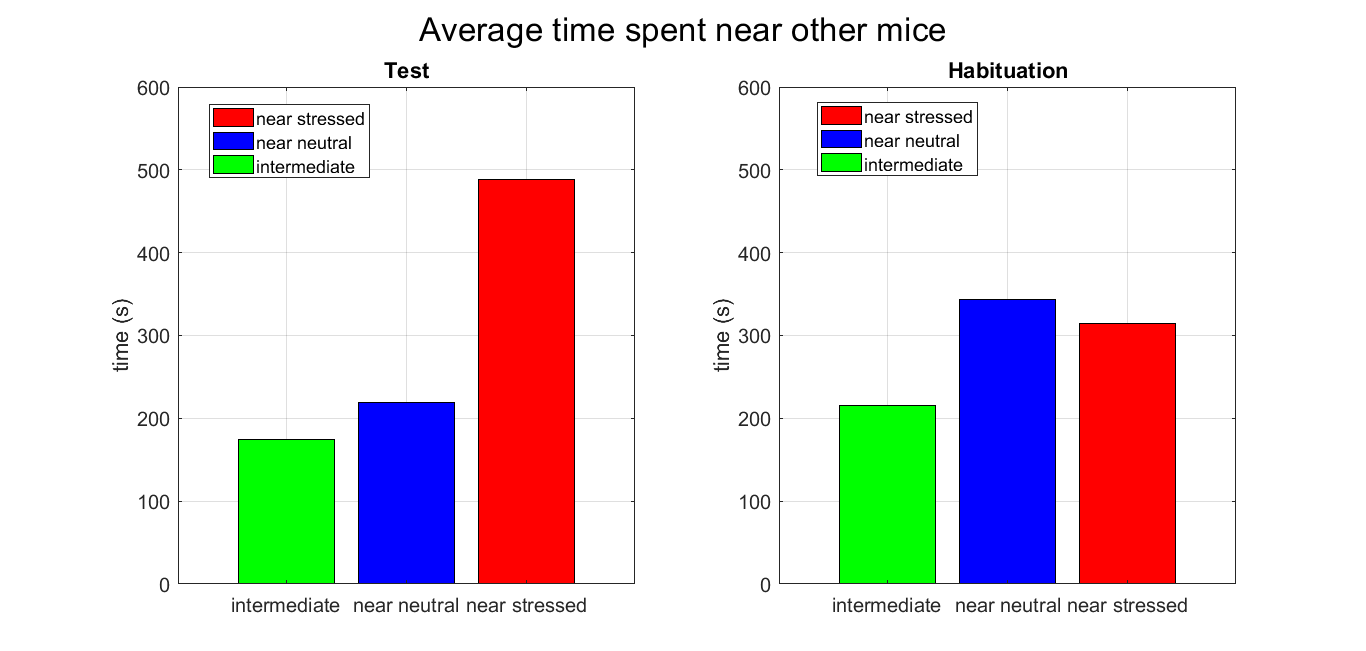
\includegraphics[scale=.42]{times.png} 
		%\end{center} 
		\caption{\textit{Average time spent by the observer near the demonstrator cages, or in the intermediate area. Left: results during the test. Right: results during the habituation. }}
		
	\end{figure}
	
In the work of [Scheggia-Managò], the same neuronal population, namely the somatostin interneurons, had been observed during a task following a similar protocol of the current emotion discrimination task. In that case, however, the area of interest was the medial prefrontal cortex, and the main focus on the activity was in electrophyisiology. As results, it was evident that the observer mouse spent more time near the stressed demonstrators, and its neural activity (in terms of action potentials) showed higher values in those periods.\\
As for the current work, similar analyses produced the following results:

\begin{itemize}
	\item The observer spent a significantly higher time near the stressed demonstrators, rather than near the neutral one or in an intermediate zone (see Figure). Moreover, in order to rule rule that this effect was due to spatial factors present in the area in which the stressed mouse was located, a comparison with the habituation has been performed. During the habituation, the observer is free to move in the arena for the same time of the test, but in the arena the two cages for the demonstrators are empty. The results show clearly that in this situation the observer doesn't show a particular tendency for proximity, and in particular spend considerably less time near the cage of the stressed mouse.
	
	\item As for the calcium activity, no evidence of correlation seemed to emerge: from the recorded neurons, the observer mantains an overall similar average activity through the different areas of the arena. As for the demonstrators, only the neutral appears to show an increase activity during the sniffing with the observer.
	\\
	
	Next, a comparison on the average activity of mice during the phases of the task have been taken into account (see Figure). The results showed that, in general, the mean activity seems to be higher during the habituation. This happens in particular for the stressed mouse, coherently with the fact that during the habituation, it is being subjected to the stress protocol (forced restrainment), for which it is expected to show higher activity. Overall, the neutral mouse shows smaller values of calcium activity, both during habituation and test, compared to the observer and the stressed conspecifics.
	
\end{itemize}
	
	
		\begin{figure}[H]
		
		\begin{center}
			\hspace*{-1.6cm}
			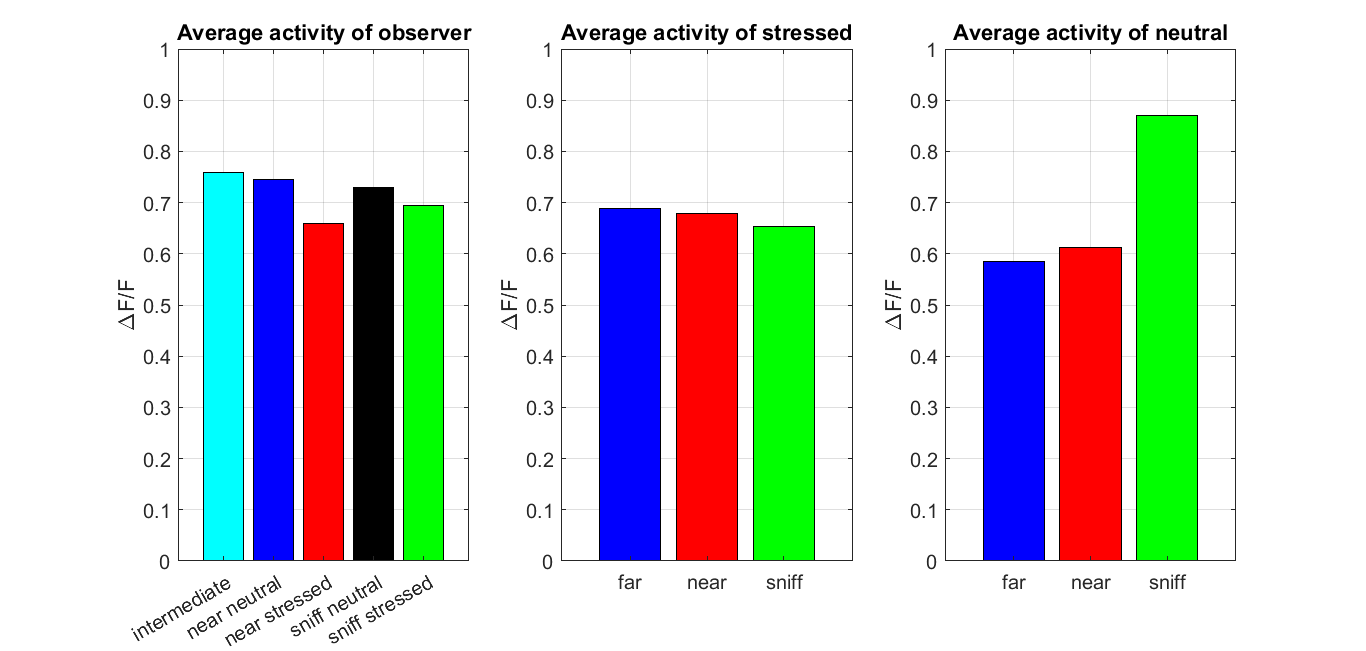
\includegraphics[scale=.42]{activity_barplot.png} 
		\end{center} 
		\caption{\textit{Average activity showed by the mice. Left: observer. No tendencies seem to emerge when it is in intermediate area, close to demonstrators or sniffing with demonstrators. Center: stressed. No tendencies seem to emerge comparing the periods when the observer is far, near or sniffing the stressed Right:neutral. During the sniffing with the observer, its activity shows higher values}}
		
	\end{figure}


\begin{figure}[H]
	
	\begin{center}
	
		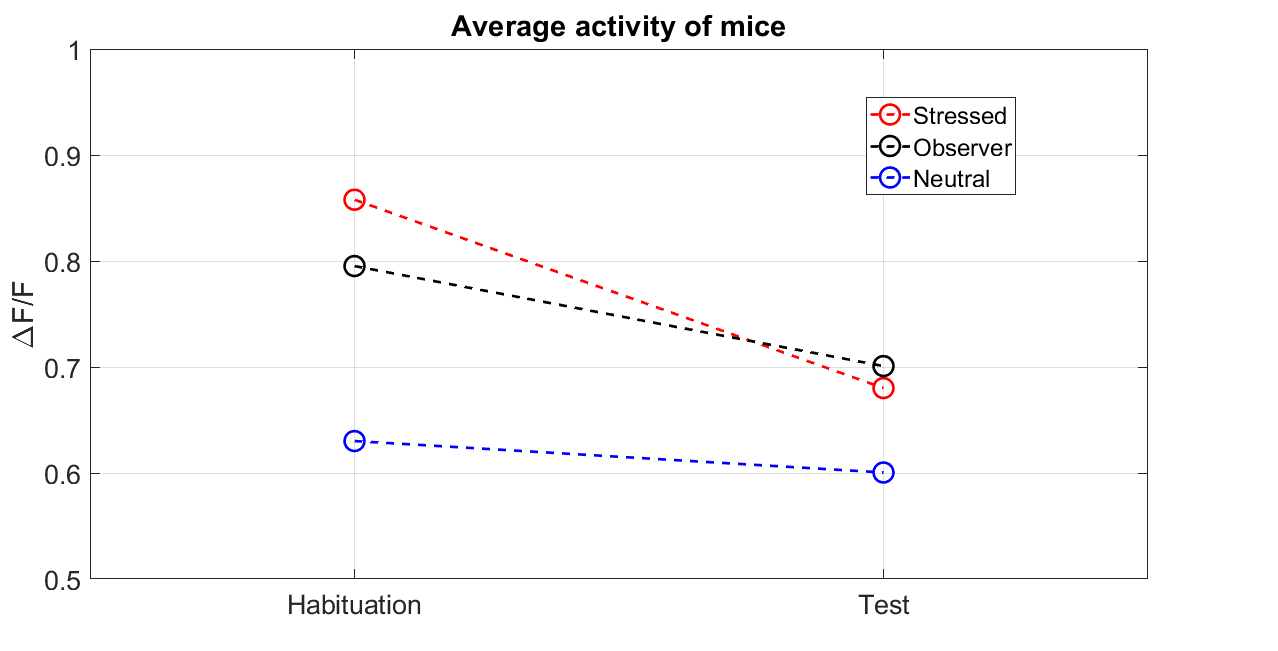
\includegraphics[scale=.4]{activities.png} 
	\end{center} 
	\caption{\textit{Evolution of the average activity of the three mice from the habituation to the test}}
	
\end{figure}


\subsection{Cross-correlation analysis for the mean activity}

\begin{figure}[H]
	
	\begin{center}
		\hspace*{-1.4cm}
		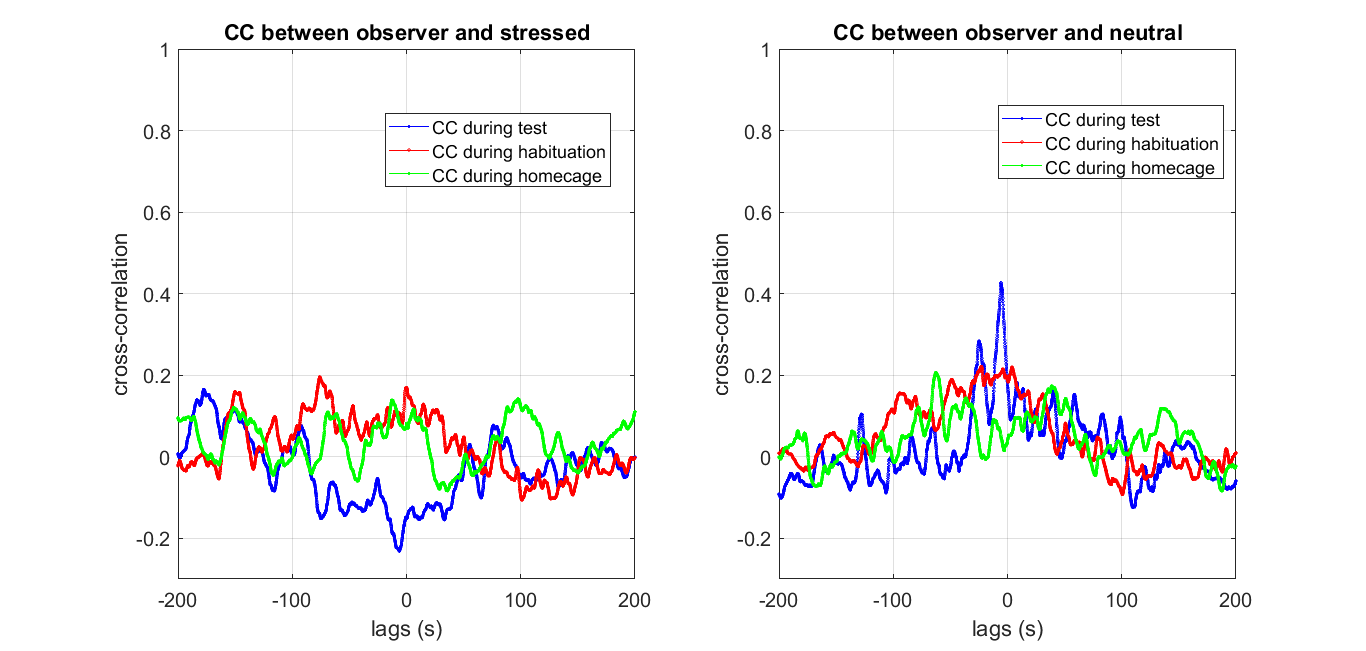
\includegraphics[scale=.4]{average_cc.png} 
	\end{center} 
	\caption{\textit{Left: average cross-correlation between observer and stressed. Right: average cross-correlation between observer and neutral}}
	
\end{figure}

With the \textit{Interbrain analysis}, we wonder whether the interactions of two mice are followed by a synchronization of their neural signals. As explained in Section 2.2, one of the main tool for the synchronization analysis is the \textbf{cross-correlation}.\\
As first step, following the approach of [Kingsbury], every mice has been gifted with its \textit{overall activity}, consisting in a mean of the activities of all its recorded neurons. Such activities can be considered in several parts:

\begin{enumerate}
	\item Restriction to the times of proximity between the observer and the stressed
	\item Restriction to the times of proximity between the observer and the neutral
	\item Restriction to the times of reciprocal sniffing between two mice
\end{enumerate}

so that we can analyze the correlation between the activities of two mice when they are actually close to each other. In this context, a cross-correlation analysis on the mean activity has been performed, comparing what happens during the homecage, habituation and test (see Figure). During homecage and habituation phases, the three mice are kept separate. Therefore, inspecting the correlation between the activites during these phases is a useful \textit{control}, i.e. a case of comparison in order to see what to expect when correlation should not be present.
\\

As first analysis, an overall activity of the inspected ROI has been considered. A mean of all the $\frac{\Delta F}{F}$ signals in each neurons has been computed for every mice, and subdivided in the parts defined by 1-3. Next, the cross correlation between observer and stressed and observer and neutral mean activies has been computed as described in (ref chap 2). As shown in Figure, analyzing the average cross correlation between the two experiments one can notice the presence of a peak around $ lag=0 $ for the pair observer-neutral in the test phase. This tendency is not present in the control cases of habituation and homecage, making it proper of the test. On the other side,the cross correlation between observer and stressed does not show any particular difference with respect to the homecage and habituation ones. A further control has been given by observing the cross correlation between the observer and one demonstrator considering the periods when the observer was visiting the other demonstrator. As result, the cross correlation between observer and neutral is abolished considering the instants when the observ was visiting the stressed, and the cross correlation between observer and stressed remains non signficative when the observer is visiting the neutral. Overall, these results may show the presence of a synchronization between neural activities between the observer and the neutral mouse, but not between the observer and the stressed, and this effect is present only during the test and during the proximity of the two mice.\\
Next, two particulr cases have been considered: the sniffing interactions and the first part (2 minutes of the test). The sniffing is known to be one of the most direct interactions that two mice can display between each other, and therefore is of a particular interest for what could happen at synchronization level. The restriction to the first two minutes of the test is of interest based on previous results [Kingsbury], which show that the first periods of interactions between mice is the one which determine the most some relevant neural tendency, such as synchronization. The results obtained showed the following (Figure):

\begin{itemize}
	\item The result during the sniffing interactions are coherent with the ones obtained during the whole test: a peak around $lag=0$ is present only in the cross corelation computed between observer and neutral, but not oberver and stressed
	
	\item In consistence with previous results, the peak of cross correlation between observer and neutral is higher if we restrict the analysis to the first two minutes of interaction. A visual confirmation of the improve in synchronization in the test rather than habituation in this case is given by Figure
	
\end{itemize}

A summary of the cross-correlation results can be see in Figure. For every case, the values refer to the cross-correlation peak recorded around $lag=0$. While for the observer-stressed case no particular difference arise, between observer and neutral the test phases show higher correlations, in particcular thr sniffing and the beginning of the test.

\begin{figure}[H]
	
	\begin{center}
		\hspace*{-1.4cm}
		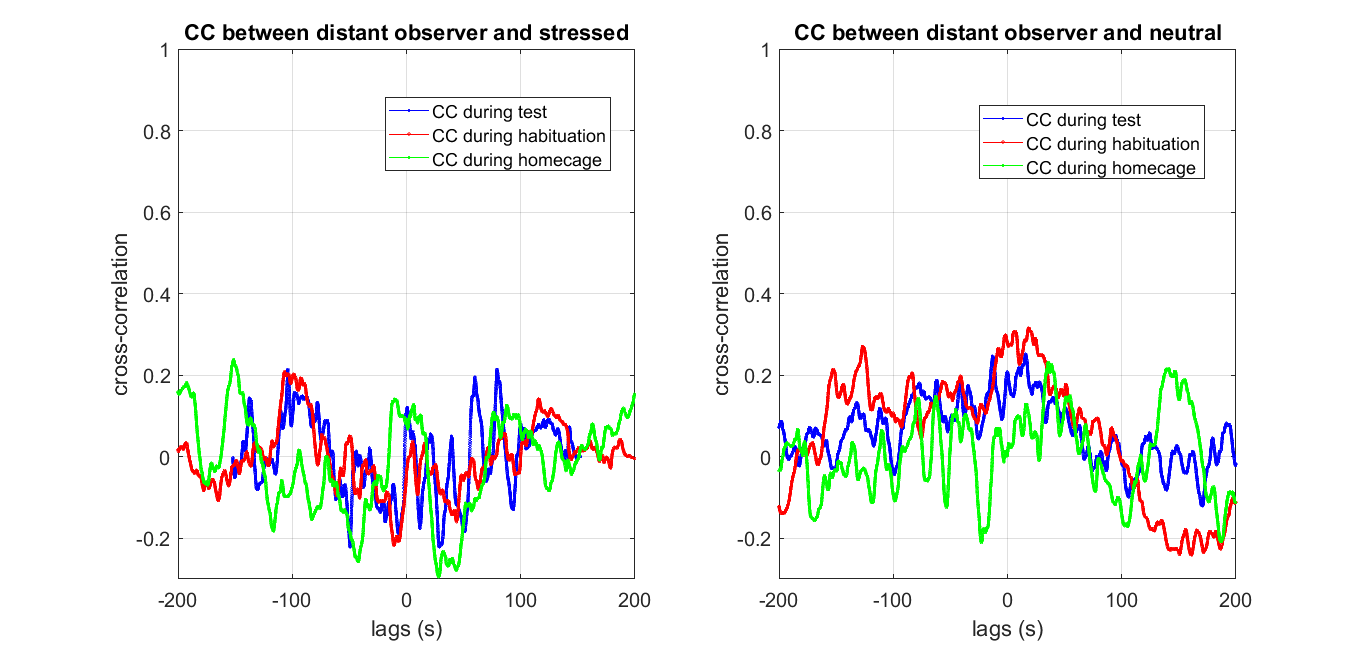
\includegraphics[scale=.4]{cc_distant.png} 
	\end{center} 
	\caption{\textit{Left: average cross-correlation peaks between observer and stressed when observer is visiting neutral. Right: average cross-correlation peaks between observer and and neutral when observer is visiting stressed.}}
	
\end{figure}

\begin{figure}[H]
	
	\begin{center}
		\hspace*{-1.4cm}
		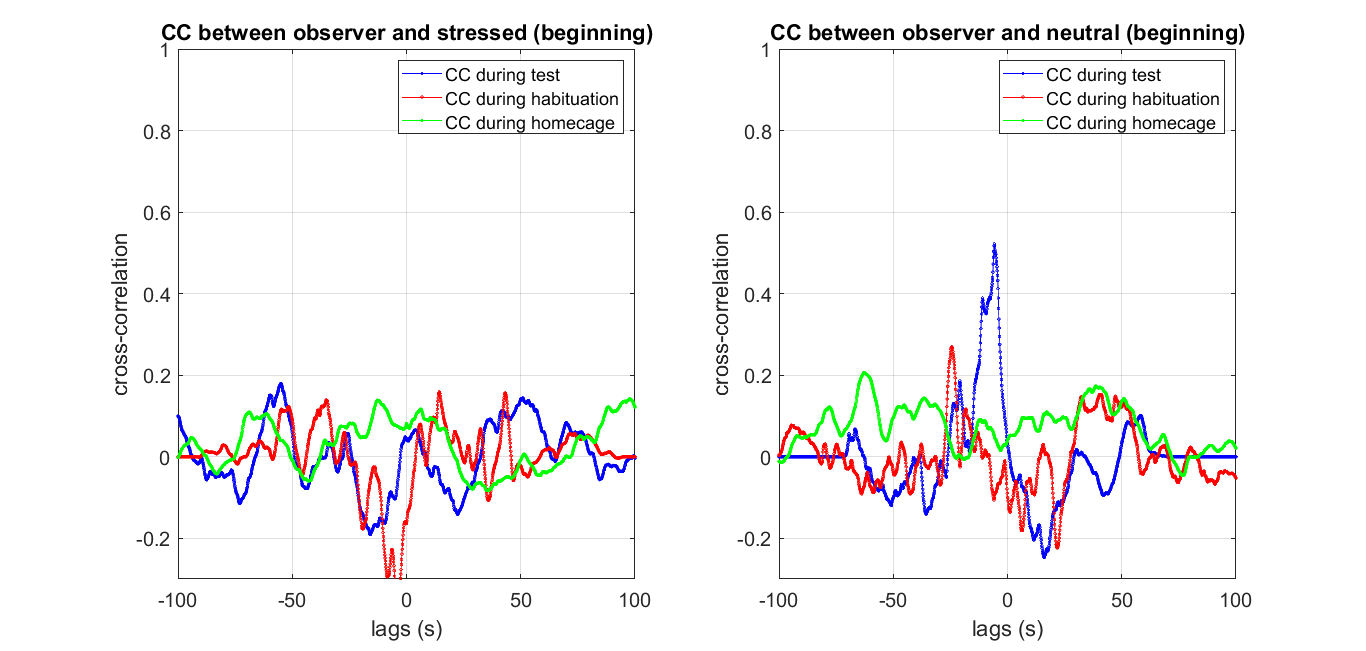
\includegraphics[scale=.4]{average_cc_initial.png} 
	\end{center} 
	\caption{\textit{Left: average cross-correlation between observer and stressed, during the first two minutes of test. Right: average cross-correlation between observer and neutral, during the first two minutes of test.}}
	
\end{figure}

\begin{figure}[H]
	
	\begin{center}
		\hspace*{-1.4cm}
		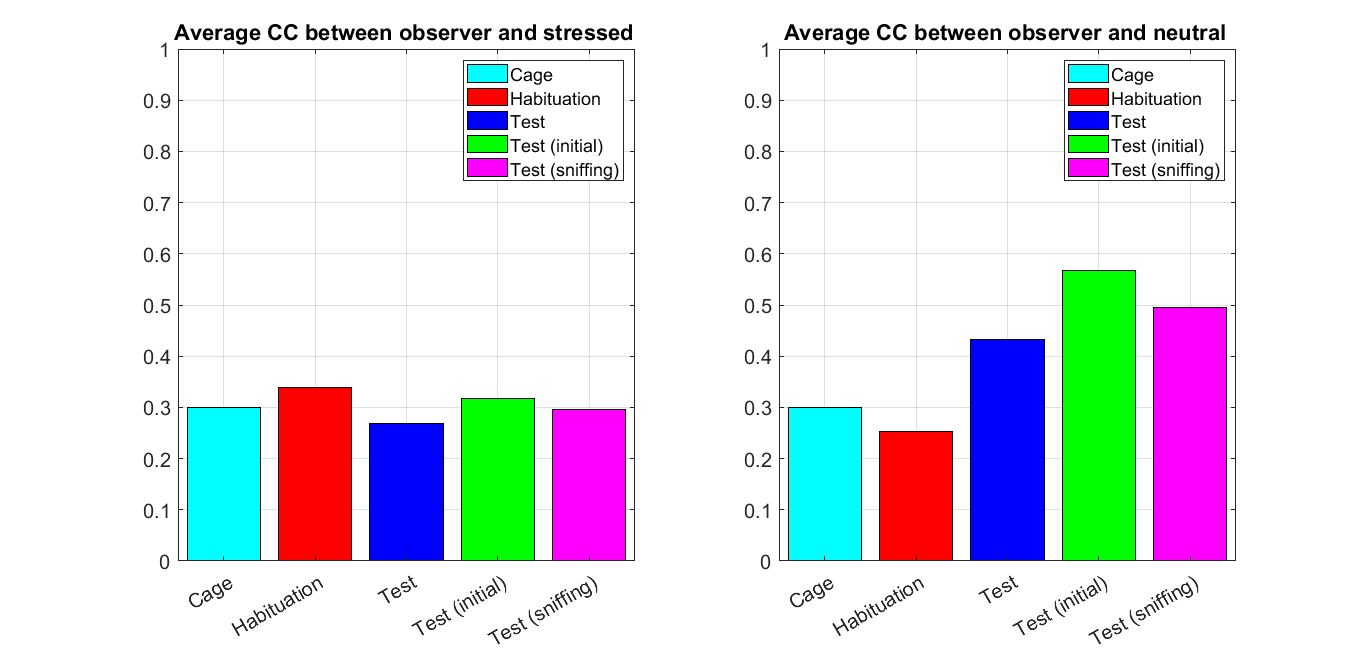
\includegraphics[scale=.4]{cc_average.png} 
	\end{center} 
	\caption{\textit{Left: average cross-correlation peaks between observer and stressed. Right: average cross-correlation peaks between observer and and neutral.}}
	
\end{figure}

\end{document}
